%!TEX program = lualatex
\documentclass[aps,prl,twocolumn,groupedaddress,amsmath,amssymb]{revtex4-1}

% Math and stuff
\usepackage{amsmath,amssymb,amstext}
\usepackage{mathtools}
\usepackage{bbm} % indicator function \mathbbm{1}
\usepackage[no-math]{fontspec}
\setmainfont[Ligatures={TeX}]{Linux Libertine O}
\usepackage[libertine, cmintegrals]{newtxmath}
\usepackage{microtype}
\usepackage{amsfonts}

% Language, right quotes
\usepackage{polyglossia}
\setmainlanguage{english}
\usepackage{csquotes}



% Page geometry
\usepackage{geometry}

%% Images, graphics, drawings
%\usepackage{pgfplots}
\usepackage{tikz}
\usetikzlibrary{patterns,positioning,calc}
\usepackage{xcolor}
\usepackage[font=small,format=plain,labelfont=bf,up,textfont=it,up]{caption}
\usepackage{subcaption}
\usepackage{graphicx}

\usepackage{todonotes}
\usepackage{siunitx}

% Citing and linking
%\usepackage[style=alphabetic,backend=bibtex]{biblatex}
\usepackage{hyperref}

\usepackage{xparse}

% math ops
\newcommand{\td}[1]{\mathrm{d}#1}
\newcommand{\dt}{\mathrm{d}t}
\newcommand{\pdiv}[2]{\frac{\partial #1}{\partial #2}}
\newcommand{\tdiv}[2]{\frac{\td{#1}}{\td{#2}}}
\newcommand{\definemapping}[3]{#1\colon #2 \ \longrightarrow\  #3\,}
\newcommand{\ix}[1]{_{\mathrm{#1}}}

\DeclareMathOperator{\const}{const}
\DeclareMathOperator{\sign}{sg}
\DeclareMathOperator{\argmin}{argmin}
\DeclareMathOperator{\argmax}{argmax}
\newcommand{\transpose}{^{\mathrm{T}}}

\newcommand{\uniform}[1]{\mathcal{U}\left( #1 \right)}
\newcommand{\mat}[1]{\mathbf{#1}}

\NewDocumentCommand{\functional}{mmo}{%
  #1 %
  \IfValueTF{#3}{_{#3}}{}%
  \!\left[ #2 \right]%
}

\NewDocumentCommand{\expectation}{om}{\functional{\mathbb{E}}{#2}[#1]}
\NewDocumentCommand{\probability}{om}{\functional{\mathbb{P}}{#2}[#1]}
\NewDocumentCommand{\variance}{om}{\functional{\mathbb{V}}{#2}[#1]}


\newcommand{\reals}{\mathbb{R}}
\newcommand{\pihalf}{\frac{\pi}{2}}
\newcommand{\sigmaalg}{\mathcal{F}}
\newcommand{\borel}{\mathcal{B}}


\begin{document}

    \title{Supplementing U-Nets with a GAN Loss for Cell Segmentation}
    \author{Erik Schultheis}
    \maketitle

	\section{Introduction}

    In this work a deep network called a U-Net \cite{ronneberger2015u} is used to generate
    segmentations from cell images. This means that given a black and white microscopy image of a
    slice of cells, we want the  network to detect the cell boundaries even if the quality of the
    original image is very low. To improve upon that architecture a regularizing loss inspired by
    generative adversarial  networks is added.

    The U-Net architecture was chosen due to its success for other bioimaging segmentation tasks. 
    It allows for precise localization of the segmentation classes and can be trained from few
    training examples. It is fully convolutional so it can be applied independent of the input
    image size. However, even the production of the low number (order of hundreds) of labelled
    training data can be expensive. 

    An alternative that does not need paired training data can be constructed with generative
    adversarial networks. In this case a \emph{Generator} network constructs fake data, and a
    \emph{Discriminator} network tries to distinguish it from real data. The competing  processes
    between generator and discriminator result in the generator producing more and more realistic
    data.

    By changing the generator to an image to image network, and introducing a cycle consistency
    loss, this architecture can be used for image-to-image transfers as done e.g. in
    \emph{CycleGANs} \cite{zhu2017unpaired} and \emph{DiscoGANs} \cite{kim2017learning}.  The
    training requires data from both domains, but does not need paired samples. In particular, one
    can use a data set that contains cell images for which no corresponding ground-truth
    segmentation is available.
    
    Unfortunatle, the training process of GAN networks is far more unstable and slow than that of 
    U-Nets. For this reason we try to combine these two processes by adding a GAN-like loss as an
    additional regularization to the U-Net. This should make the U-Net produce pictures that are 
    both close to the ground-truth data given a pixel-wise loss, and that are accepted as realistic
    by the discriminator.

    In the following we first build up the U-Net training process, taking a look at the effects
    of data augmentation, the choice of loss function, and the U-Net architecture. Then the GAN
    discriminator is introduced and calibrated so that it actually improves the training. This 
    turned out to require quite careful tuning of the discriminator parameters. We then look at the
    effects that the additional regularization has on the sample efficiency of the U-Net. Finally, 
    some shortcomings of the current approach are discussed and an outlook on possible future work 
    is given.

    \section{U-Net}

    In this section the basic U-Net model upon which the discriminator loss extension will be based,
    is developed. Several experiments are performed to find good settings for data augmentation, the
    loss function and the network architecture. Due to the high amount of hyperparameters, a
    comparison of all possible settings is not possible. Instead, one aspect (number of layers,
    loss function, data augmentation pipeline, \ldots) is varied and optimized while the others are
    kept fixed.

    \subsection{Architecture}
    The U-net architecture consists of resolution decreasing downward blocks, followed by resolution
    increasing upwards blocks. To improve the spatial precision, each upward block gets  as input
    both the result of the preceding block, and that of the corresponding downward block at the same
    resolution. As a downward block two convolutions with $3\times3$ receptive field are followed by
    a $2\times2$ max-pooling. With each deeper layer the  number of feature maps doubles. The
    convolutions are padded such that the resulting feature map has the same resolution as the
    original one.

    When increasing the spatial size of a feature layer by deconvolutions, the network is
    prone to generate so-called checkboard artifacts \cite{odena2016deconvolution}. While the 
    supervised nature of the U-Net training suppressed these problems, we still investigate whether
    performance can be improved by using a model inherently resistent to these effects. For that
    the deconvolutions are replaced by an upscaling, followed by a regular convolution. 

    The effects of different network depths (measured as the number of downward convolution blocks),
    and the choice of upscaling instead of deconvolution, are shown in figure~\ref{fig:arch}. As the
    results are only marginally different, the depth-4 upscaling network is chosen, as it may have
    additional, unused modelling capacity that could become useful when the additional loss is
    introduced below.

    \begin{figure}[tbp]
        \begin{subfigure}[c]{\linewidth}
            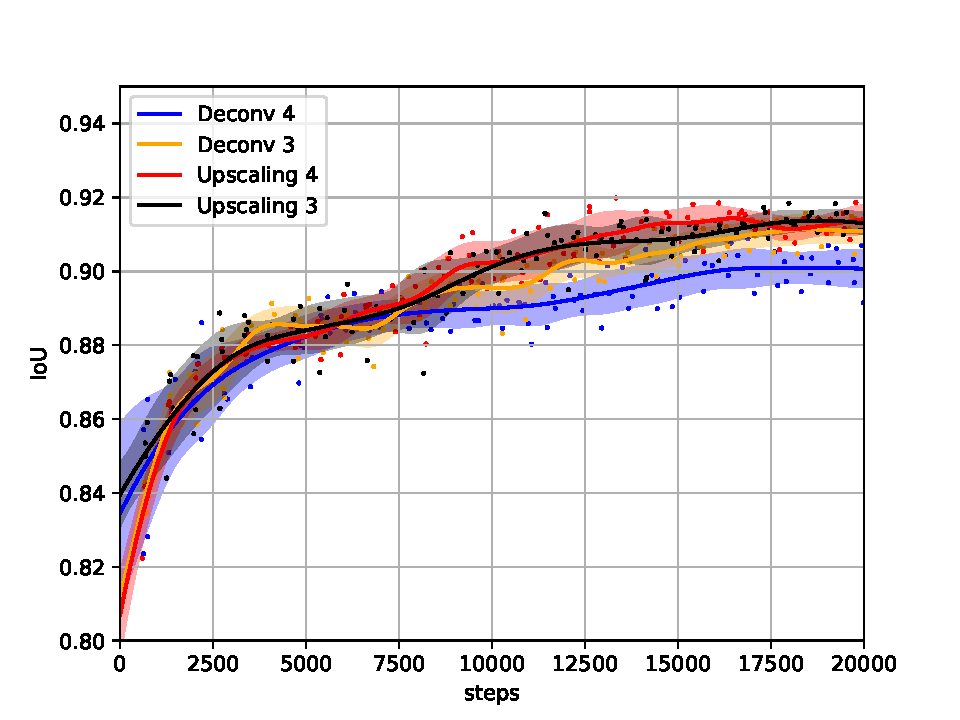
\includegraphics[width=\linewidth]{figures/arch.pdf}
            \caption{IoU}
        \end{subfigure}
        \begin{subfigure}[c]{\linewidth}
            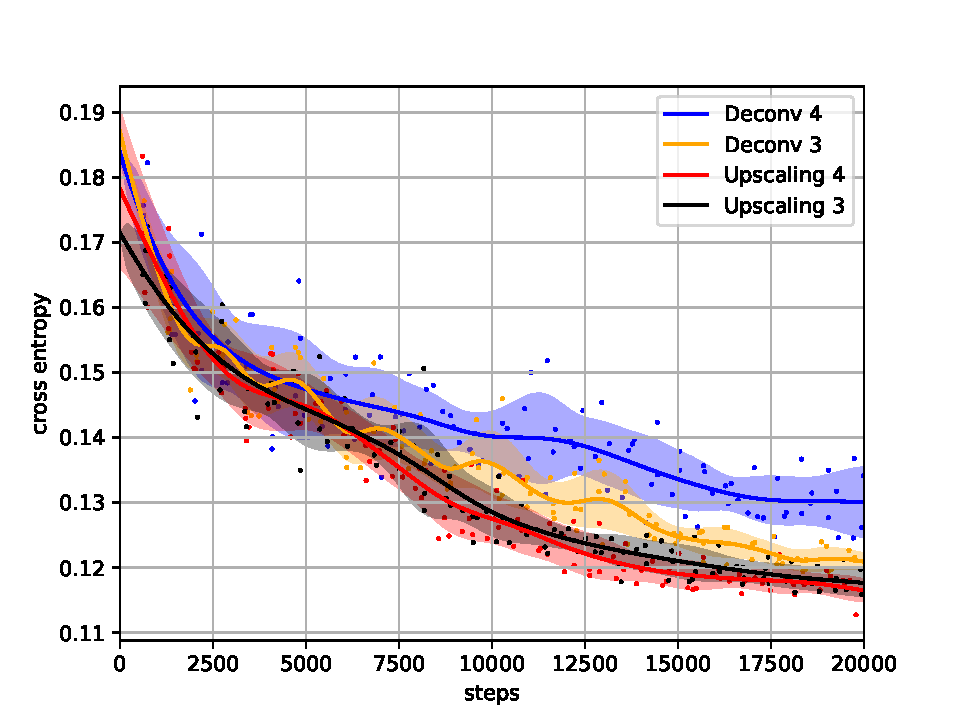
\includegraphics[width=\linewidth]{figures/arch_xent.pdf}
            \caption{Cross-entropy}
        \end{subfigure}
        \caption{Comparison of different network architectures in terms of segmentation IoU and
        cross entropy. The performance of the different settings is comparable, except for the 
        4 layer deconvolution network. This may indicate an overfitting problem that can be
        prevented by either less parameters (depth 3) or by imposing additional structure on the 
        generation process (upscaling). The training loss is cross entropy and full data
        augmentation as described in the text has been used.}
        \label{fig:arch}
    \end{figure}

    \subsection{Data augmentation}
    Since there are only very few cell images and corresponding segmentations avaiable it is 
    necessary to make heavy use of data augmentation to facilitate training and generalization 
    of the network. The training data consists of 118 pairs of images, the evaluation data contains
    28 image pairs.

    The original cell images are given as 512 by 512 grayscale pixels. To reduce memory consumption
    these images are randomly cropped to $256\times256$. To increase the training set the images are
    randomly flipped (left-right and up-down) and rotated by multiples of 90 degrees, and the
    variability is further increased by random reductions of the image contrast by a factor in the
    range $[0.25, 1]$. These images are then downsampled to $128\times128$ to reduce the class
    imbalance. For cell images this corresponds to a $2\times2$ average pooling, whereas the binary
    segmentation images are resized with max pooling to preserve the binary structure.

    The positions of the cell boundaries may not be specified pixel-precise by the cell images. To 
    penalize shifts of the order of a few pixels not as much as missing boundary classification, one 
    can replace to hard, binary classification ground truth with a slightly blurred version (
    Gaussian filter with $\sigma=1$). To ensure that the central portion of the cell boundary still
    gets classified as $100\%$ cell boundary, the original ground truth is added to the blurred 
    version, with the result clipped at $1$.

    An even stronger increase in image variability can be archieved when the changes in contrast are
    not applied homogenously to the image (in which case they can mostly be reverted by an  image
    standartization), but with a locally varying strength. For this a 16 by 16 mask is created and
    upscaled to the full image size, blurred, and then used to interpolate between the image and a
    version whose contrast has been reduced to $10\%$ of the original value. The same approach can
    be used to apply local variations in image brightness. An example can be seen in
    figure~\ref{fig:augmentimage}.

    The effectiveness of this augmentation is demonstrated in figure~\ref{fig:augment}. Note that we
    cannot directly compare the effects on the evaluation loss, as the blurring of segmentations
    affects the loss calculation.

    \begin{figure}[tbp]
        \begin{subfigure}[c]{0.45\linewidth}
            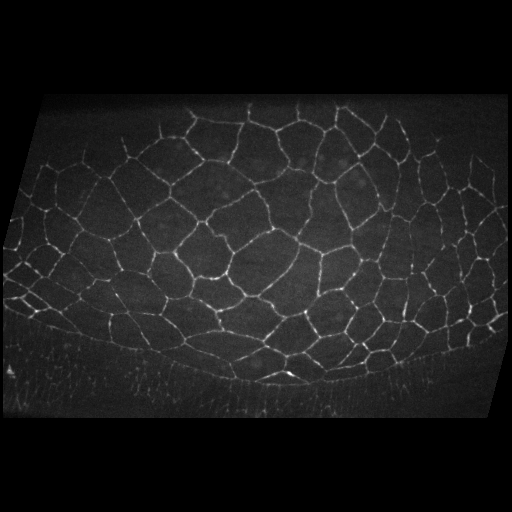
\includegraphics[width=\linewidth]{figures/original.png}
            \caption{original}
        \end{subfigure}
        \begin{subfigure}[c]{0.45\linewidth}
            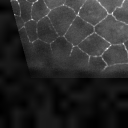
\includegraphics[width=\linewidth]{figures/augmented.png}
            \caption{preprocessed}
        \end{subfigure}
        \caption{Result of applying the full preprocessing procedure to a cell image. 
        Notice the brighter and darker patches caused by local contrast and brigthness changes.}
        \label{fig:augmentimage}
    \end{figure}

    \begin{figure}[tbp]
        \begin{center}
        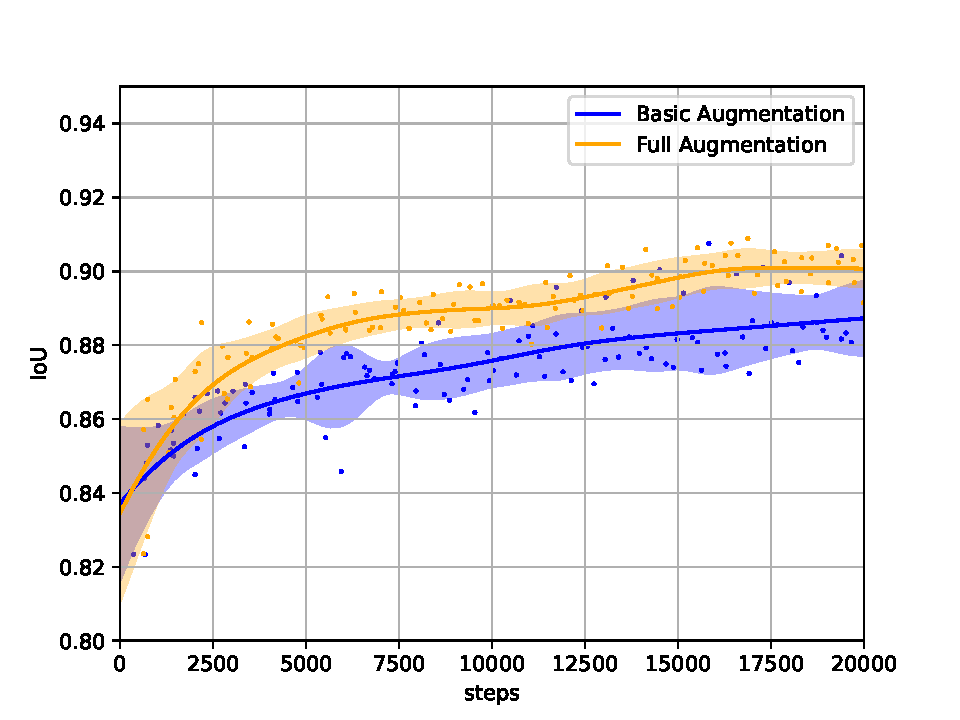
\includegraphics[width=\linewidth]{figures/augment.pdf}
        \end{center}
        \caption{Effects of more extensive data preprocessing (additional blurring and local 
        contrast/brightness variations) vs only simple (crop, flip, rotate) augmentations on the 
        IoU of the generated segmentations over the learning process.}
        \label{fig:augment}
    \end{figure}

    \subsection{Loss function}
    A second design decision for the training process is the choice of the loss function. 
    Interpreting the segmentations as probability maps for a pixel being on a cell boundary frames
    this task as a pixel classification problem and leads to a pixelwise binary (sigmoid) cross 
    entropy loss. Thinking of the problem as an image-to-image transfer would suggest a pixelwise
    mean squared error as a simple loss function. 

    In both cases the strong class imbalance constitutes a problem: Most pixels in the target 
    segmentations are black, so a network that outputs all-black images would already get a high 
    accuracy. This can be countered by giving more weight to white pixels, which is automatically 
    done in the following way: The percentage of white $\bar{w}$ in the image is calculated 
    and the loss at a pixel of value $p$ is weighted as $w = p/\bar{w} + (1-p)/(1-\bar{w})$. If there
    are 9 times more black pixels than white, $\bar{w}=0.1$ and white pixels are weighted 9 times 
    stronger than black pixels.

    As demonstrated in figure~\ref{fig:mse} the cross-entropy and mse based training do perform
    about equally. Their difference is significantly smaller than the variability between runs. In
    the following we will use the cross-entropy loss, allowing for a probabilistic interpretation
    of the resulting segmentations.

    \begin{figure}[tbp]
        \begin{center}
        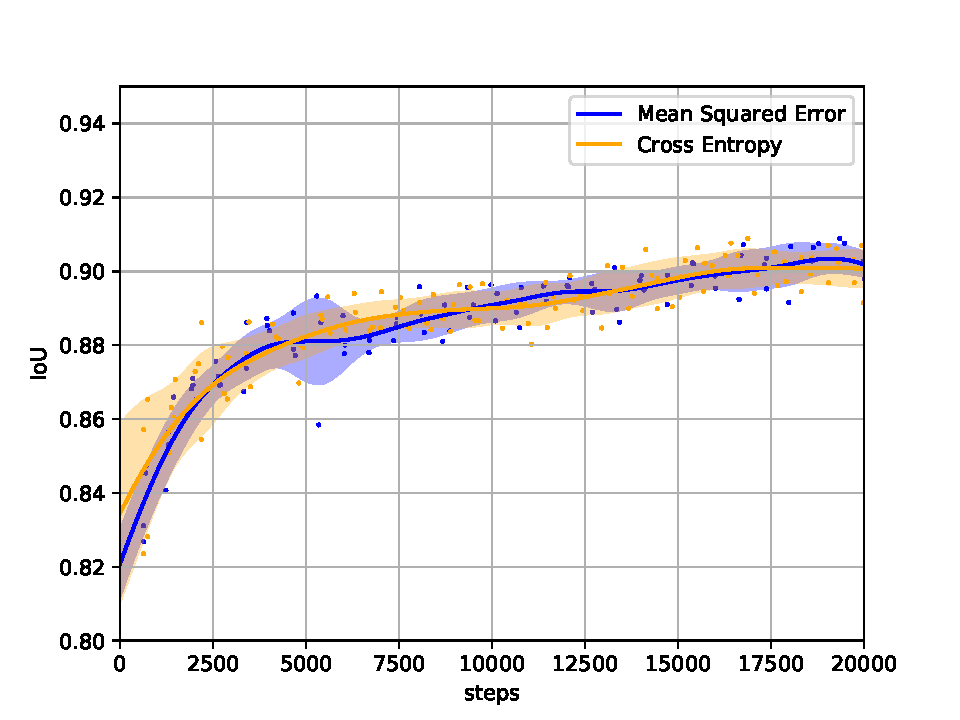
\includegraphics[width=\linewidth]{figures/mse.pdf}
        \end{center}
        \caption{Comparison of learning progress using the cross entropy and mean squared error 
        losses. White pixels (cell boundaries) are weighted more strongly than black pixels. 
        Within the given error bounds, both loss functions result in equivalent performance.}
        \label{fig:mse}
    \end{figure}

    \section{Regularisation by Discriminator}

    \subsection{Architecture}
    \begin{figure}[tbp]
        \begin{center}
        %\tikzstyle{neuron} = [draw, circle, text centered, text width=0.75cm, minimum height=0.5cm, fill=white]

\pgfdeclarelayer{background}
\pgfdeclarelayer{foreground}
\pgfsetlayers{background,foreground}

\begin{tikzpicture}[node distance=1.5cm, auto]
    \begin{pgfonlayer}{foreground}
        \node (A) {$A$};
        \node [below of=A] (B) {$B$};
        \node [right of=A] (unet) {UNet};
        \node [right of=unet] (fake) {$B^{\prime}$};

        \node [right of=fake, circle, fill=white, yshift=-0.8cm] (disc) {D};
        \node [right of=disc, yshift=0.6cm, xshift=-0.5cm] (fakec) {$d_{\mathrm{g}}$};
        
        \node [right of=disc, yshift=-0.6cm, xshift=-0.5cm] (realc) {$d_{\mathrm{r}}$};
        \node [right of=realc, xshift=-0.5cm] (Ldr) {$L_{\mathrm{d, r}}$};

        \node [above of=fakec] (Lgc) {$L_{\mathrm{g, c}}$};
        \node [right of=fakec, xshift=-0.5cm] (Ldf) {$L_{\mathrm{d, f}}$};

        \node [draw, circle, inner sep=1.0pt] (Ld) at ($(Ldr)!0.5!(Ldf)$) {$+$};

        \node [above right=0.4cm and 0.0cm of fake.east] (xent) {$L_{\mathrm{U}}$};
        \node at (xent|-Lgc) [draw, circle, fill=white, inner sep=1.0pt] (Lg) {$+$};

    \end{pgfonlayer}

    \begin{pgfonlayer}{background}
        % Data flow: UNet path
        \draw[->] (A) -- (unet) -- (fake);
        \draw[->] (fake) -- (fake|-xent) -- (xent);
        \draw[->] (xent|-B) -- (xent);
        \node at (xent|-B) [circle,fill,inner sep=1.0pt]{};
        \draw[->] (xent) -- (Lg);

        % Data flow: Generator path
        \draw[->] (fake) -- ([xshift = -0.5cm]disc.center|-fake);
        \draw[->] ([xshift=0.4cm]disc.center) -- (fakec);
        \draw[->] (fakec) -- (Lgc);
        \draw[->] (fakec) -- (Ldf);

        % Data flow: Discriminator path
        \draw[->] (B) -- ([xshift = -0.5cm]disc.center|-B);
        \draw[->] ([xshift=0.4cm]disc.center) -- (realc);
        \draw[->] (realc) -- (Ldr);
        \draw[->] (Ldr) -- (Ld);
        \draw[->] (Ldf) -- (Ld);
        

        % The UNet Symbol
        \draw[fill=white] (unet) -- ++ (-1, -0.9) -- ++ (0, 1.8) -- (unet);
        \draw[fill=white] (unet) -- ++ (+1, -0.9) -- ++ (0, 1.8) -- (unet);

        \draw [->] (unet) ++ (-0.5, +0.5) -- ++ (1, 0);
        \draw [->] (unet) ++ (-0.5, -0.5) -- ++ (1, 0);

        % The discriminators
        \draw[fill=white] (disc) ++ (+0.5, 0) -- ++ (-1, -1.0) -- ++ (0, 2.0) -- cycle;
       
        \draw (Ld.east) -- ++ (0.2, 0) -- ++ (0, -1.1) -- ++ (-1.8, 0);
        \draw[->, thick] (Ld.east) ++ (-1.6, -1.1) -- ([xshift=-0.7cm, yshift=0.3cm]disc.center);
    \end{pgfonlayer}

    % The update lines need to be in the foreground
    \begin{pgfonlayer}{foreground}
        \draw (Lgc.west) -- ([xshift=0.5cm]unet|-Lgc.west);
        \draw[->, thick] ([xshift=0.5cm]unet|-Lgc.west) -- ++ (-1.7, -1.7);

        % for some reason this needs to be redrawn here!
        \node at (xent|-Lgc) [draw, circle, fill=white, inner sep=1.0pt] (Lg) {$+$};
    \end{pgfonlayer}

\end{tikzpicture}
        \end{center}
        \caption{Architecture of the U-Net. Bold arrows indicate weight updates by gradient descent. 
        The U-Net loss $L\ix{U}$ is based on a (pixel wise) comparison of $B$ and $B^{\prime}$. The
        discrimination losses are based on the discrimination results $d\ix{r} = D(B)$, 
        $d\ix{g}=D(B^{\prime})$. They are $L\ix{g, c} = \mathrm{xent}(d\ix{g}, 1)$, 
        $L\ix{d, f} = \mathrm{xent}(d\ix{g}, 0)$ and $L\ix{d, r} = \mathrm{xent}(d\ix{r}, 1)$.}
        \label{fig:unet_dics}
    \end{figure}
    
    The U-Net architcture above is now supplemented with a discriminator network to further refine
    the generated segmentations as shown in figure~\ref{fig:unet_dics}. The disciminator follows the
    architecture used in DCGANs \cite{dcgan}, i.e. it consists of blocks of a convolution followed
    by BatchNorm followed by a leaky ReLU. Since the U-Net is fully convolutional and thus can act
    on input images of arbitrary size, it made sense to also construct a fully convolutional
    discriminator, which is achieved by the last layer being a global average pooling into a single
    unit.

    As we want to train the discriminator on images that look somewhat realistic, 
    we only start training it after having trained the U-Net for 500 steps. The generator loss, in 
    turn, is only sensible for a sensible discriminator, so this additional loss is only enabled 
    after 750 steps. 

    The loss function for the generator consists of a cross entropy loss that makes the generator
    try to fool the discriminator, and a feature matching loss that tries to ensure that the
    features in the hidden layers of the discriminator follow the same statics (in this case mean),
    independently of whether the input comes from a real segmentation of from a generated one
    \cite{salimans2016improved}. The effect of the feature matching loss can be seen in 
    figure~\ref{fig:gan_fm}. 

     \begin{figure}[tbp]
        \begin{center}
        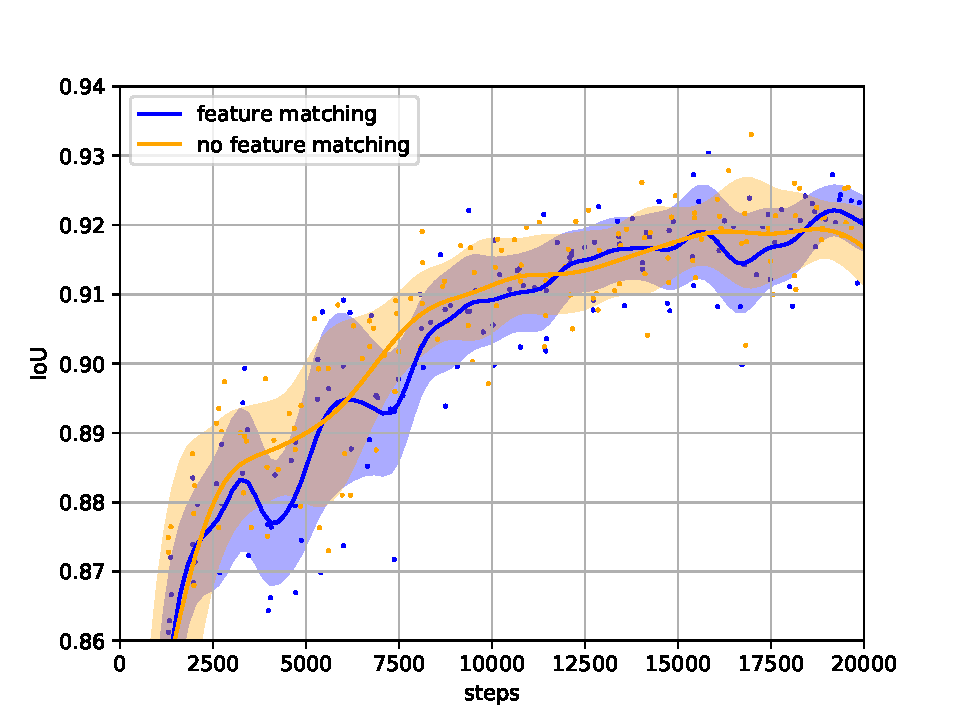
\includegraphics[width=\linewidth]{figures/gan_3_no_fm.pdf}
        \end{center}
        \caption{Comparison of learning progress with and without feature matching for the three
        layer UNet-GAN model. The differences between these two approaches are smaller than the 
        variability in different runs.}
        \label{fig:gan_fm}
    \end{figure}

    This loss is weighted with a factor $\lambda$ and then added to the pixel-wise U-Net loss for 
    training of the U-Net parameters.

    \subsection{Stabilizing the Training}

    Unfortunately the discriminator training can be very unstable, as the training process
    depends on a balance between discriminator and generator performance. This can be seen in 
    figure~\ref{fig:gan_3_opt} where the optimizer of the discriminator is varied.

    \begin{figure}[tbp]
        \begin{center}
        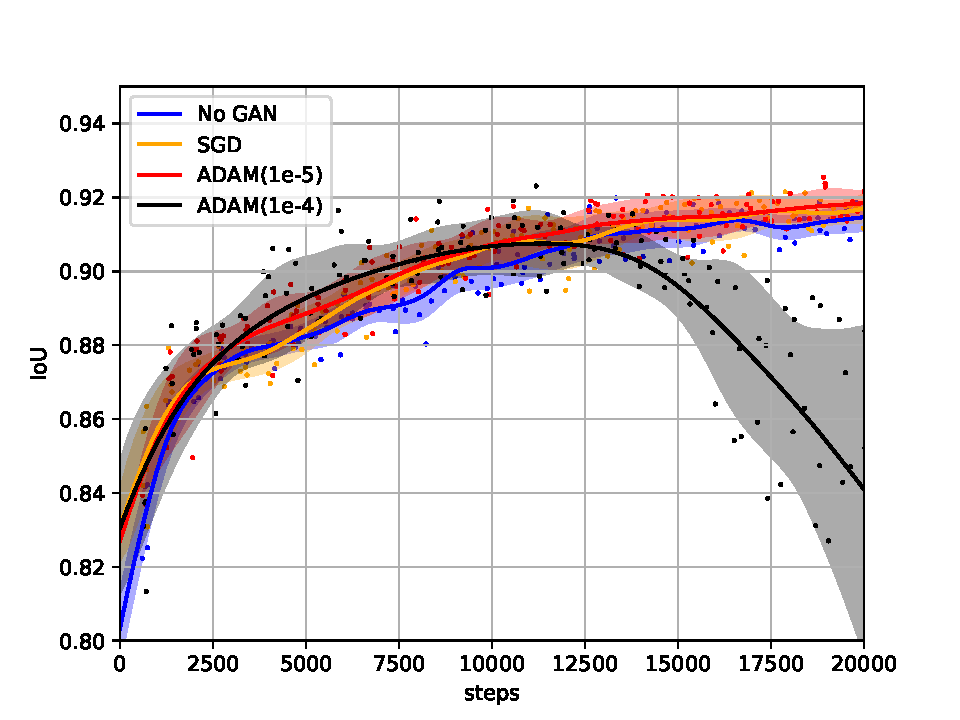
\includegraphics[width=\linewidth]{figures/gan_3_opt.pdf}
        \end{center}
        \caption{Learning progress for the three block GAN with different optimizers for the
        discriminator subnetwork. If this is configured properly, the GAN leads to a slight increase
        in performance compared to the pure U-Net. However, if the discriminator is learning too 
        fast, performance deteriorates severely. Not, however, that during earlier stages of learning,
        the strongly learned discriminator actually outperforms the other approaches.}
        \label{fig:gan_3_opt}
    \end{figure}

    That the decline in performance is actually a consequence of discriminator and generator getting
    out of balance is demonstrated in \autoref{fig:gdloss}. 

    \begin{figure}[tbp]
        \begin{center}
        \begin{subfigure}[c]{\linewidth}
        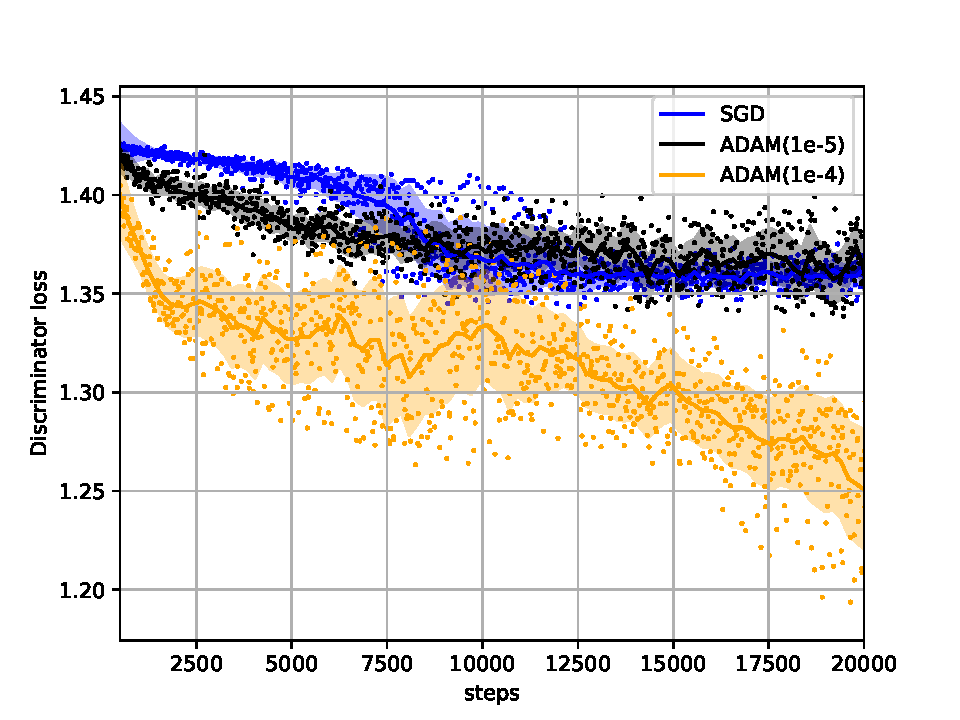
\includegraphics[width=\linewidth]{figures/dloss_opt.pdf}
        \label{Discriminator loss}
        \end{subfigure}
        \begin{subfigure}[c]{\linewidth}
        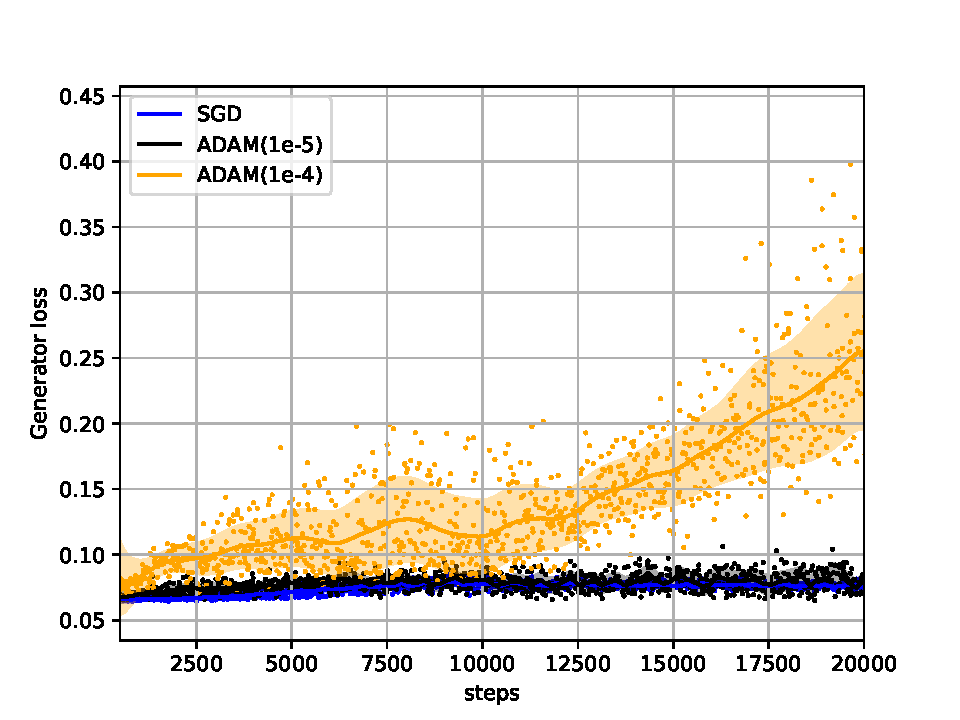
\includegraphics[width=\linewidth]{figures/gloss_opt.pdf}
        \label{Generator loss (logarithmic scale)}
        \end{subfigure}
        \end{center}
        \caption{Comparison of generator and discriminator losses. If the discriminator learns 
        too fast, it manages too decrease its loss faster than the generator learning can improve
        the images to fool the discriminator. Then the discriminator loss keeps decreasing, causing
        a perpetual increase in the generator loss. This, in turn, results in disuptive changes
        to the learning process.}
        \label{fig:gdloss}
    \end{figure}

    Taking a look at the generated images \autoref{fig:unet_vs_ganunet}
    reveals another problem: A strong GAN loss seems to cause severe artifacts
    in the generated image. Adding the GAN causes the cell boundaries to
    appear sharper. However, at strong GAN contribution these lines also start
    to appear at locations where no cell boundary is present.

    \begin{figure}[tbp]
        \begin{subfigure}[c]{0.45\linewidth}
            \includegraphics[width=\linewidth]{figures/27_orig.png}
            \caption{Cell image}
        \end{subfigure} %
        \begin{subfigure}[c]{0.45\linewidth}
            \includegraphics[width=\linewidth]{figures/27_seg.png}
            \caption{Cell boundaries}
        \end{subfigure} \\
        \begin{subfigure}[c]{0.45\linewidth}
            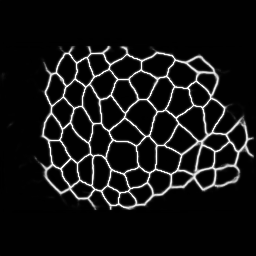
\includegraphics[width=\linewidth]{figures/27-00.png}
            \caption{$\lambda=0$}
        \end{subfigure}%
        \begin{subfigure}[c]{0.45\linewidth}
            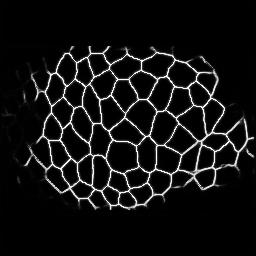
\includegraphics[width=\linewidth]{figures/27-15.png}
            \caption{$\lambda=0.15$}
        \end{subfigure}\\
        \begin{subfigure}[c]{0.45\linewidth}
            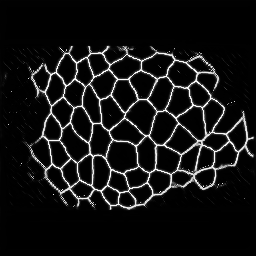
\includegraphics[width=\linewidth]{figures/27-25.png}
            \caption{$\lambda=0.25$}
        \end{subfigure}%
        \begin{subfigure}[c]{0.45\linewidth}
            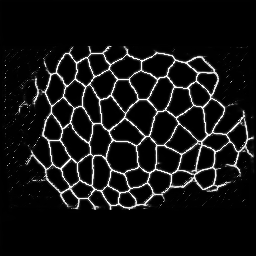
\includegraphics[width=\linewidth]{figures/27-33.png}
            \caption{$\lambda=0.25$}
        \end{subfigure}
        \caption{Comparison of resulting image for the U-Net ($\lambda=0$) and U-Net with GAN loss.
         The additional discrimination loss causes the segmented cell boundaries
        to become more crisp, but also adds some artifacts. These images show that the improvement 
        in IoU is not due to a qualitatively better segmentation approach, but due to the better 
        matching of cell areas resulting from the sharper boundaries.}
        \label{fig:unet_vs_ganunet}
    \end{figure}

    Looking at the resulting learning curves \autoref{fig:gan_up} shows that adding the GAN does
    result in an imporved IoU. However, this does not seem to be caused by detecting more cells, but
    by refining the cell boundaries. At this point, it is important to note that the ground truth
    data used here does not have segmentations for ``difficult'' to see cells. Thus, the network
    learning to detect those would actually result in a lower IoU and higher loss.

    \begin{figure}[tbp]
        \begin{center}
        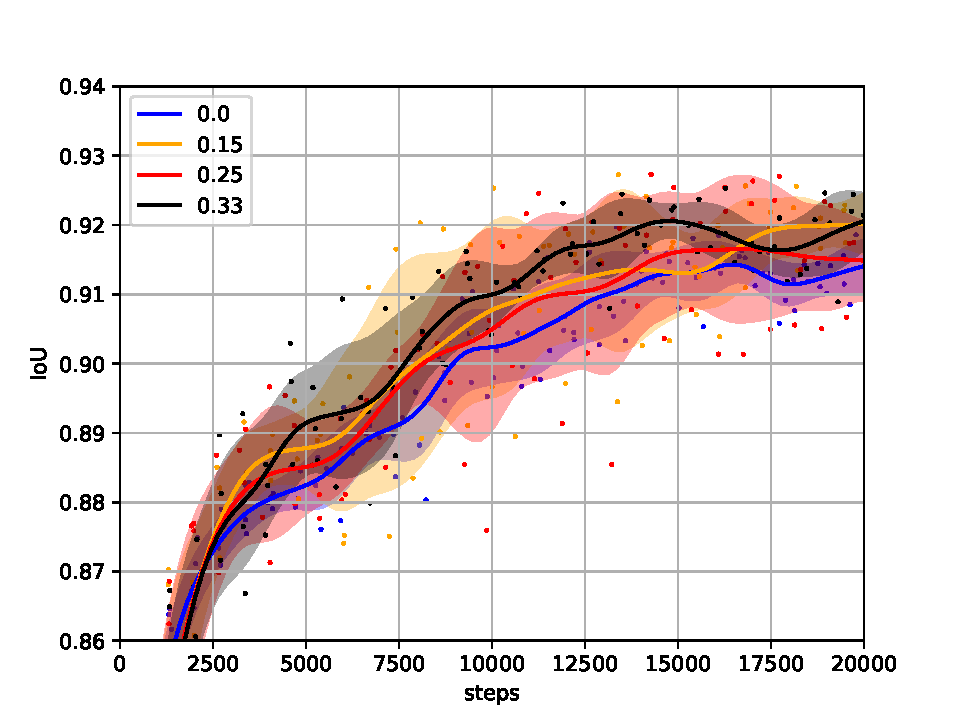
\includegraphics[width=\linewidth]{figures/gan_4_w.pdf}
        \end{center}
        \caption{IoU over training time for different GAN loss factors $\lambda$. Generally, introducing the
        GAN loss does improve the IoU. However, as the pictures in \autoref{fig:unet_vs_ganunet} suggest, 
        this does not always indicate a better segmentation.}
        \label{fig:gan_up}
    \end{figure}


    \section{Sample Efficiency}

    A first experiment in sample efficiency can be performed by reducing the training set to only 20
    images. This drastic reduction to about one sixth of the original training data is handled
    rather well by the U-Net approach. While the IoU becomes significantly reduced, it still remains
    above $84\%$. The performance levels out after a few thousand steps, whereas for the full data
    set the training needs about 20000 steps to complete.

    Adding the GAN loss improves the results slightly, see \autoref{fig:reduced_data}. This is in
    line with the previous results that the GAN training improves the stroke of the cell boundaries,
    but does not help in detecting more cells.  Note that the same hyperparameters as for the full
    dataset were used; no fine tuning was performed.

    \begin{figure}[tbp]
        \begin{center}
        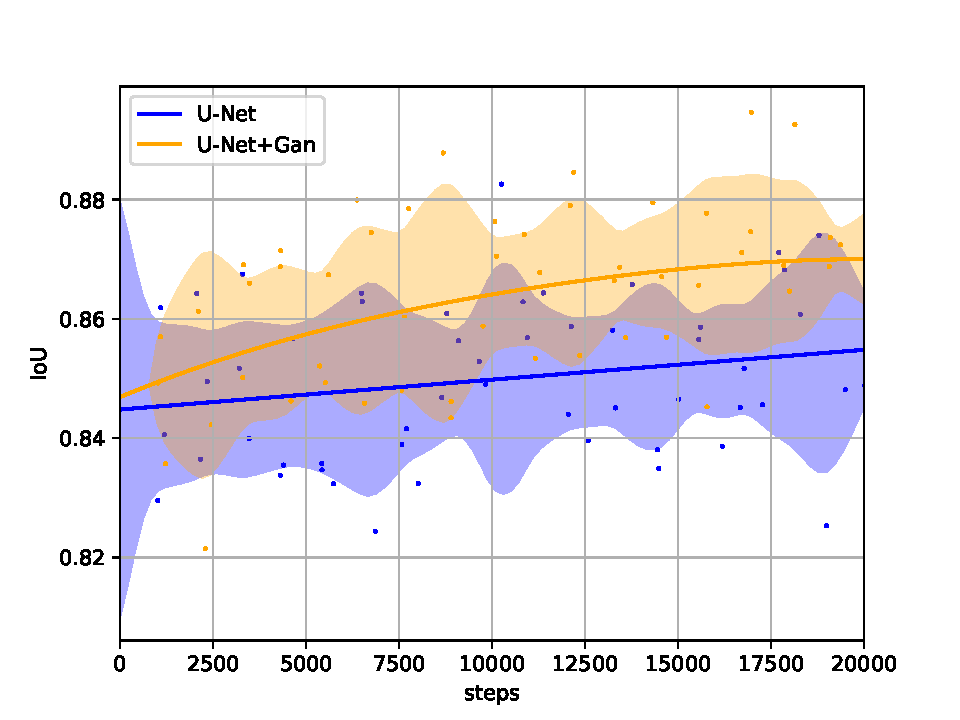
\includegraphics[width=\linewidth]{figures/less_data.pdf}
        \end{center}
        \caption{IoU when training only on 20 examples, with and without GAN loss. For reference
        also the behaviour on the full training set is shown. In this scenario the additional GAN
        loss provides some improvement.}
        \label{fig:reduced_data}
    \end{figure}


    \section{Discussion and Further Work}

    A significant problem in training and evaluation the segmentations is due to the quality of the
    ground truth data. As the network becomes good it starts to (correctly) mark more cell
    boundaries at the outer fringes of the cell image. However, these lines are not part of the
    ground-truth data (because the quality of the original image in these regions is really low), so
    the cross-entropy loss will train the network to not detect these boundaries. See for example
    the left side of the images in \autoref{fig:unet_vs_ganunet}.

    This could be alleviated by providing an additional map that contains information about the
    condidence of the ground truth data -- so that the cross entropy could be weighted less in low
    confidence regions. For the evaluation procedure this means that it is impossible for the loss
    to become smaller (or the IoU larger) than some threshold that is determined by the data
    quality.

    Another possible area of improvement is the data augmentation pipeline. The current
    augmentations have the advantage of transforming the segmentations pixel precise. If one lifts
    this restriction, arbitrary rotations and shears, as well as slight scale variations, could be
    added as preprocessing modifications.

    The problem of the GAN favouring hard boundaries, independently of whether a cell exists in the
    original image at the given position, might be tackled by including the microscopy image in the
    discriminator. Then the decision of whether a segmentation looks acceptable would be conditioned
    on the given input image.

    As above demonstrated, the GAN loss can be used to improve the training when there are only few
    training examples. Going even further, one could modify the training procedure to only require
    partially labeled data. For any data point for which no ground truth segmentation exists, the
    U-Net should still generate a segmentation that the discriminator accepts as ``realistic''.


    \section{Summary}

    A U-Net can be used to detect cell boundaries in microscopy images. By aggressive data
    augmentation the training can be improved. Introducing an additional discriminator loss that
    judges produced segmentations for whether the seem ``realistic'' can further improve the
    networks performance, but requires some fine-tuning and makes the training process more
    unstable. In a setting where labelled data is extremely scarce, the regularisation provided by
    the discriminator becomes more useful.




    \bibliographystyle{plain}
    \bibliography{lit.bib} 
\end{document}

